\documentclass[a4paper]{article}
\usepackage{amsfonts}
\usepackage{amsmath}
\usepackage{amssymb}
\usepackage{graphicx}	

\begin{document}
  
\noindent \large Auteur: Joe Ayoub \\
\noindent \large Studierichting: Informatica\\
\noindent \large Oefeningenreeks 3G nr.11.1 \\

\medskip

\normalsize


$f(x)  = \dfrac{2x}{x^2 + 1}$ \\

V.A: $\lim\limits_{x \rightarrow 0} \dfrac{2x}{x^2 + 1} = 0$  geen V.A \\

H.A: $\lim\limits_{x \rightarrow \infty} \dfrac{2x}{x^2 + 1} = 0$  T.O \\

\begin{tabular}{c|ccc}
	$x$ &  & $0$ & \\ \hline
	$f(x)$ & $-$ & $0$ & $+$ \\
\end{tabular} \\

Dus: \\
Als $x \rightarrow +\infty$ dan is de limiet $0^+$ \\
Als $x \rightarrow -\infty$ dan is de limiet $0^-$ \\

$f'(x) = 2 \cdot \left(\dfrac{x}{x^2 + 1 }\right)'$ \\

$ = 2 \cdot \dfrac{(x^2 + 1) \cdot 1 - 2x^2}{(x^2 + 1)^2}$ \\

$ = 2 \cdot \dfrac{-x^2 + 1}{(x^2 + 1)^2} = \dfrac{-2(x^2 - 1)}{(x^2 + 1)^2}$ \\


$f''(x) = -2 \cdot \left(\dfrac{x^2 - 1}{(x^2 + 1)^2}\right)'$ \\

$ = -2 \cdot \dfrac{(x^2 + 1)^2 \cdot 2x - 4x(x^2 + 1)(x^2 - 1)}{(x^2 + 1)^4}$ \\

$ = -2 \cdot \dfrac{(x^2 + 1) \cdot (2x(x^2 + 1) - 4x(x^2 - 1))}{(x^2 + 1)^4}$ \\

$ = -2 \cdot \dfrac{(2x(x^2 + 1 - 2x^2 + 2)}{(x^2 + 1)^3}$ \\

$ = \dfrac{4x(x^2 - 3)}{(x^2 + 1)^3}$ \\ \\

Nulpunten van:
\begin{itemize}
	\item $f(x) = \{0\}$
	\item $f'(x) = \{-1, 1\}$
	\item $f''(x) = \{-\sqrt{3}, 0, \sqrt{3}\}$
\end{itemize}

\begin{tabular}{c|ccccccccccc}
	$x$ &  & $-\sqrt{3}$ &  & $-1$ &  & $0$ &  & $1$ &  & $\sqrt{3}$ & \\ \hline 
	$f(x)$ & $-$ & $-$ & $-$ & $-$ & $-$ & $0$ & $+$ & $+$ & $+$ & $+$ & $+$ \\ 
	$f'(x)$ & $-$ & $-$ & $-$ & $0$ & $+$ & $+$ & $+$ & $0$ & $-$ & $-$ & $-$ \\
	$f''(x)$ & $-$ & $0$ & $+$ & $+$ & $+$ & $0$ & $-$ & $-$ & $-$ & $0$ & $+$ \\ \hline
	$f(x)$ & $\searrow$ & $\searrow$ & $\searrow$ & $m(1)$ & $\nearrow$ & $\nearrow$ & $\nearrow$ & $M(1)$ & $\searrow$ & $\searrow$ & $\searrow$ \\
		   & $\smile$ & B & $\frown$ & $\frown$ & $\frown$ & B & $\smile$ & $\smile$ & $\smile$ & B & $\frown$ \\
\end{tabular} \\

Coordinaten van de buigpunten:
\begin{itemize}
	\item $\left(-\sqrt{3},\dfrac{-\sqrt{3}}{2}\right)$
	\item $(0,0)$
	\item $\left(\sqrt{3},\dfrac{\sqrt{3}}{2}\right)$
\end{itemize}

Tekening: \\
\begin{figure}[h]
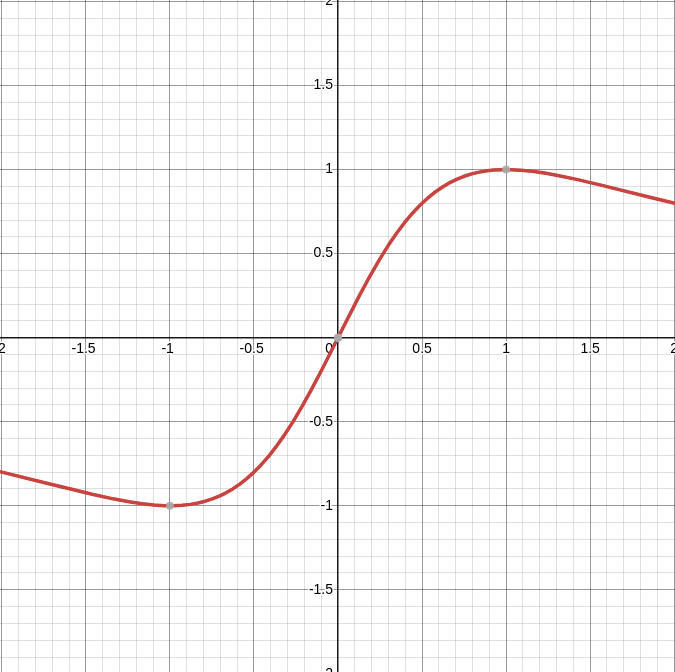
\includegraphics[width=10cm]{3G-11.1-joe.ayoub.INF.png}
\end{figure}

\begin{thebibliography}{999}
%\bibitem{a} Referentie
\end{thebibliography}
\end{document} 
